Knowledge of projective geometry is vital to understanding elliptic curves, as they are curves that are defined in the projective plane.
However, the definition is not too complicated.
\begin{definition}
	An elliptic curve is a regular, projective cubic curve.
\end{definition}
Here, a cubic simply means that the polynomial that defines the curve is of degree three.
So for example, $F(X,Y,Z) = X^3 + 2XYZ + 5YZ^2 + \frac{1}{2}Z^3$ defines an elliptic curve $F(X,Y,Z) = 0$. % Check this!!

Our interest in elliptic curves is mainly concentrated on a special property, unique to them.
It is possible to turn the set of points of an elliptic curve $E$ into a group by introducing a special addition law that satisfies all of the group axioms.
We do not prove this in this document for the sake of brevity but there are many proper treatments elsewhere, such as 
\begin{figure}[htpb]
	\centering
	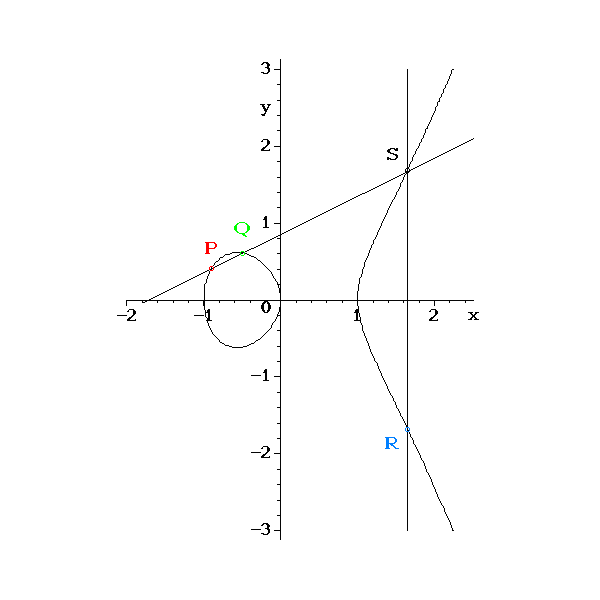
\includegraphics[scale=0.5]{addition.png}
	\caption{The chord-tangent composition law on an elliptic curve\footnote{probably a temporary diagram}}
	\label{chord-tangent}
\end{figure}

%%%%%%%%%%%%%%%%%%%%
\begin{definition}
	An elliptic curve is a non-singular cubic projective curve. For our purposes, they can all be written as $y^2 = f(x)$, where $f(x)$ is a cubic polynomial in $x$ with no repeated roots.
\end{definition}
